\chapter{Реализация и экспериментальная проверка \dots}

В этой главе описывается, что и как было запрограммировано, отлажено, 
протестировано, и что в результате получилось. Большинство работ должны 
содержать приведенные ниже разделы. Но нужно учитывать, что точный состав 
этой главы, как и других глав, зависит от специфики работы.

Фрагменты программного кода в тексте необходимо выделять при помощи команды 
\verb|\verb|. Многострочные листинги должны оформляться при помощи пакета 
\verb|listingsutf8|. Пример:

\begin{lstlisting}
# let s x y z = x z (y z);;
val s : ('a -> 'b -> 'c) -> ('a -> 'b) -> 'a -> 'c = <fun>
# let k x y = x;;
val k : 'a -> 'b -> 'a = <fun>
# let i = s k k;;
val i : '_a -> '_a = <fun>
\end{lstlisting}

Листинг \ref{lst:float-example} иллюстрирует использование выносных листингов.
Листинг \ref{lst:HelloWorld.scala} показывает пример включения внешнего файла 
в качестве листинга, в данном случае --- выносного.

\begin{lstlisting}[
  float=tb,frame=lines,label=lst:float-example,caption=Выносной листинг
]
List myList = new List();
Element myElement = new Element();
myList.Append(myElement);
\end{lstlisting}

\lstinputlisting[
  label=lst:HelloWorld.scala,
  float=tb,frame=lines,
  caption=Листинг из файла \texttt{HelloWorld.scala}
]{listings/HelloWorld.scala}

\section{Выбор инструментальных средств}

В этом разделе обосновывается выбор инструментальных средств; одним из критериев выбора могут быть какие-либо требования к разрабатываемой системе, и если этих требований много, они могут быть выделены в отдельный раздел, или же в приложение. Этот пункт не пишется, если в аналитической главе был раздел, посвященный сравнительному анализу и выбору инструментальных средств.




\section{Состав и структура реализованного программного обеспечения}

Нужно охарактеризовать реализованное ПО: является ли оно настольной программной для Windows, или веб-приложением в форме сайта/веб-сервиса, или модулем/подключаемой библиотекой, или \dots. Также нужно перечислить, из чего оно состоит: какие исполняемые файлы и их назначение, конфигурационные файлы, файлы баз данных, требования к программному и аппаратному окружению, и т.п.

Если реализованное приложение достаточно обширно, этот раздел может быть
разделен на несколько: один с общим описанием, и по одному на подсистемы самого
верхнего уровня.
\section{Результаты экспериментов}

\subsection{Эксперимент с 1 изображением}

\begin{figure}
	\centering
	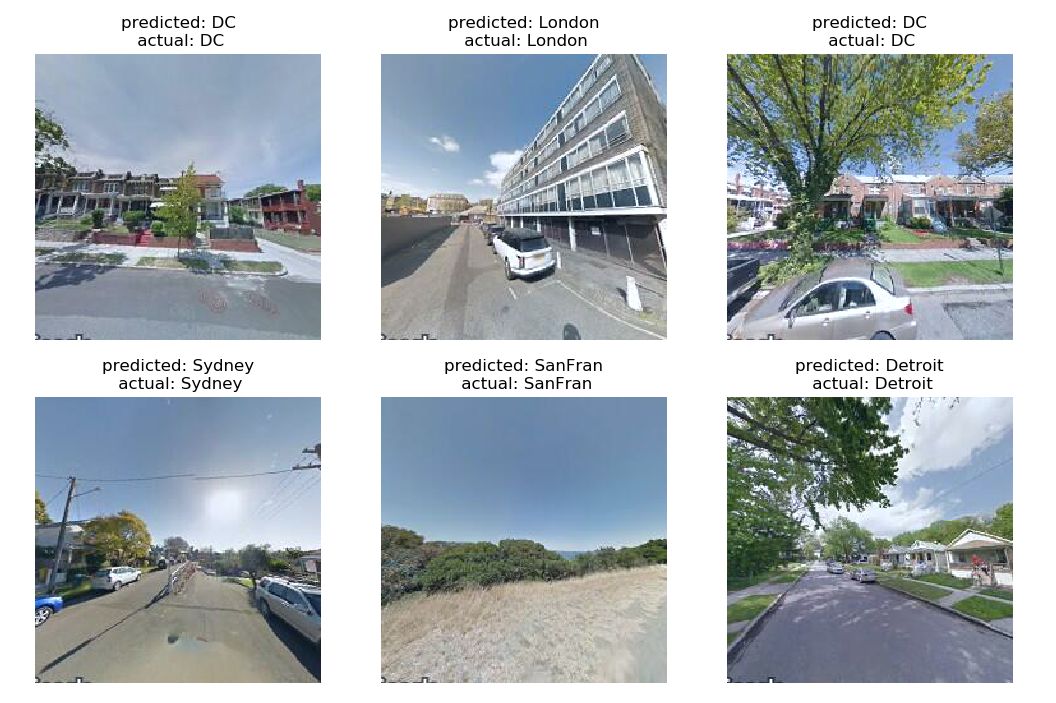
\includegraphics[width=0.9\linewidth]{res1im}
	\caption{Результат обучения модели с resNet18 по 1 изображению}
	\label{fig:res1im}
\end{figure}


\subsection{Эксперимент с альбомом} Мы сравниваем эту модель с моделью и базовый уровень, который просто усредняет прогнозы single-imagePlaNet всех изображений в альбоме и назначает
среднее для всех изображений. Усреднение в альбомах ($ \mathcal{G}= \mathbb{E}[ \mathcal{F}(X) ] $) уже
дают значительное улучшение по сравнению с одним изображением PlaNet
(45,7\% на уровне улиц), поскольку у него больше
вмятины предсказания к неоднозначным изображениям. Однако, LSTM
модель явно превосходит технику усреднения (50,5\%
относительное улучшение уровня улицы). Визуальный контроль
результатов показали, что за достоверностью следуют несколько изображений с более низким местоположением уверенность, модель LSTM присваивает низкий уровень доверия изображения, расположенные вблизи изображения с высокой степенью достоверности в то время как $ \mathcal{F} $ может «прыгать» (менять предположение о расположении альбома), модель LSTM имеет тенденцию прогнозировать близкие местоположения, кроме случаев когда есть убедительные доказательства изменения местоположения. LSTM модель работает лучше усреднения из-за того что оно присваивает всем изображениям в альбоме одинаковые уровни значимости и не может производить точные прогнозы для альбомов которые включают разные местоположения (например, альбомы поездок).

\section{Разработка тестовых примеров}

Описываются наиболее характерные тестовые примеры, для прогона на интеграционных тестах. (Да, использование unit-тестирование --- это почти всегда хорошо, основное исключение составляют работы, в которых используемый инструментарий по какой-либо причине в принципе исключает такую возможность. Например, что-нибудь вроде Mathematica.)

В этом же разделе могут приводится и результаты тестирования, включая таблицы и
графики. Результаты тестирования могут быть вынесены в отдельный раздел, если
много текстового материала и/или использована (не совсем) стандартная методика
тестирования (описание которой также нужно привести).



\section{Результаты тестирования и примеры работы системы}

Нужно помнить, что пользователем может быть не только <<менеджер>> или <<человек в белом халате>>, но и другой программист. Последнее относится, в первую очередь, к реализованным библиотекам. Для <<обычных>> приложений нередко бывают пользователи нескольких категорий --- например, обычный пользователь и администратор. Для каждой категории нужно описать, как выполняются основные функции, предпочтительно, с помощью серии скрин-шотов. Однако считается плохим тоном вставлять длинную вереницу из скрин-шотов: если их много, большую часть нужно выносить в приложение. Для \textit{этого} раздела нормальной является плотность скрин-шотов из расчета: 1 страница скрин-шотов на 1-2 страницы текста.

\textit{\textbf{Замечание.}} В ПЗ (как УИРа, так и ВКР) следует избегать ситуаций, когда значительную часть основного содержания составляют страницы с иллюстрациями и таблицами, особенно, если такие страницы следуют подряд. В основном тексте следует оставлять лишь самые основные таблицы и рисунки, а остальное --- выносить в приложение.




\section{Сравнение реализованного программного обеспечения с существующими аналогами}

В сравнении должно быть отражено, чем полученное ПО выгодно (и невыгодно) отличается от прочих ближайших аналогов. Практика показывает, что аналоги есть всегда. А если нет аналогов, значит есть частичные решения, которые реализуют какие-то части функционала вашей системы. Тут тоже может быть относительно много таблиц и графиков.



\section{Выводы}

Следует перечислить, какие практические результаты были получены, а именно: какое программное или иное обеспечение было создано. В число результатов могут входить, например, методики тестирования, тестовые примеры (для проверки корректности/оценки характеристик тех или иных алгоритмов) и др. По каждому результату следует сделать вывод, насколько он отличается от известных промышленных аналогов и исследовательских прототипов.

